\documentclass[12pt]{article}



\usepackage{amsmath}
\usepackage{subfigure}
\usepackage{amssymb}
\usepackage{gregmath}
\usepackage{cite}
\usepackage{fancyhdr}
\usepackage{url}
\usepackage{color}
\usepackage[colorlinks=true]{hyperref}
\usepackage{graphicx}
\usepackage[margin=1in]{geometry}

\graphicspath{{./pdf/}}


\begin{document}

\pagestyle{fancy}
\lhead{Gregory Ditzler}
\chead{\bfseries Rowan University}
\rhead{Advanced DSP}
\lfoot{\sf http://gregoryditzler.com}
\cfoot{  }
\rfoot{\today}
%\renewcommand{\headrulewidth}{0.4pt}
%\renewcommand{\footrulewidth}{0.4pt}


\begin{center}
  {\huge
    Introduction to Optimal Wiener Filters
  }
\end{center}




%\pagestyle{fancy}
%\lhead{Gregory Ditzler}
%\chead{\bfseries Rowan University}
%\rhead{Advanced Digital Signal Processing}
%\lfoot{\sf http://gregoryditzler.com}
%\cfoot{ \thepage }
%\rfoot{\today}






%%%%%%%%%%%%%%%%%%%%%%%%%%%%%%%%%%%%%%%%%%%%%%%%%%%%%%%%%%%%%%%
\section{Introduction \& Setup}
There are many setting where we have an input sequence $\{x[n]\}$ that consists of a desired input signal $\{s[n]\}$ which has been corrupted with undesirable additive noise $\{w[n]\}$. The goal, which is a fundamental principal in signal processing, is to filter the input signal such that the noise and interference is ameliorated from the output of the system responsible for filtering the signal. In todays lecture we shall treat the problem of filtering such a signal by estimating the presence of the additive noise. This estimation is constrained to a linear filter with an impulse response given by $\{h[n]\}$. The output of the filter produces the desired signal $\{d[n]\}$. Figure \ref{fig:lin est} shows the problem of this estimation using a linear filter. 

\begin{figure}[h!]
  \centering
  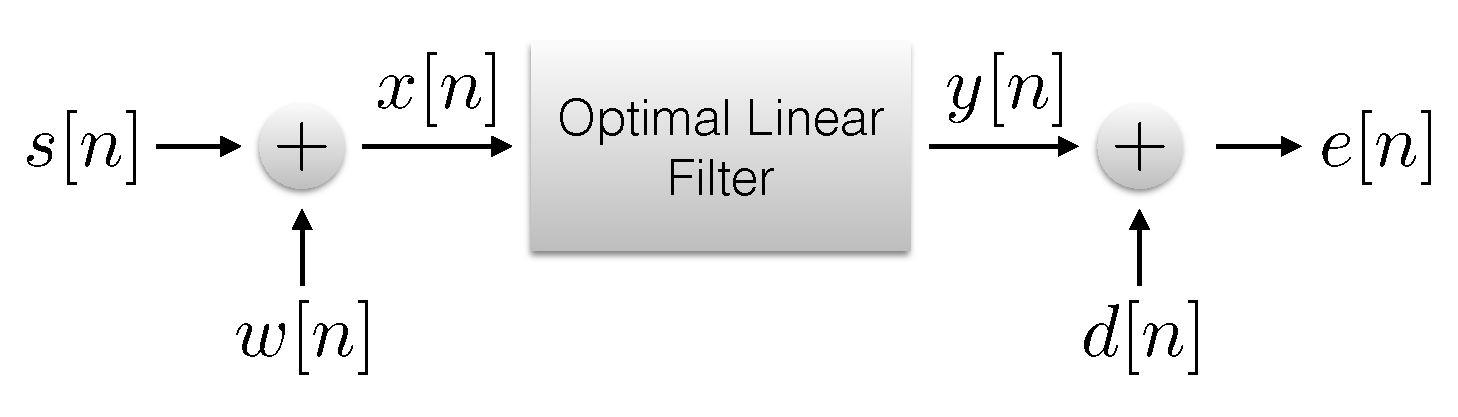
\includegraphics[width=.7\textwidth]{wiener.pdf}
  \caption{Model for a linear estimation problem. }
  \label{fig:lin est}
\end{figure}

The input signal $x[n] = s[n]+w[n]$ is presented to a linear filter with the output being given by $y[n]$. The error from this estimation is given by $e[n] = d[n] - y[n]$. There are three specific case to consider. 

\begin{itemize}
  \item If $d[n] = s[n]$ then the linear estimation problem is referred to as {\em filtering}. 
  \item If $d[n] = s[n+D]$, where $D > 0$ the problem is known as signal {\em prediction}. 
  \item If $d[n] = s[n-D]$, where $D > 0$ the problem is known as signal {\em smoothing}. 
\end{itemize}

In this lecture we focus on signal filtering and prediction. One of the central issues that we should make clear is that the user designing the filter must know the precise spectrum of the input domain to develop a precise filter. However, it is rarely the situation that the user is going to know all of these characteristics prior to building a filter. Often, we specify the filter characteristics based on some past experience, and/or trial and error. FIR/IIR design techniques can design any filter you specify -- it does not tell you whether that is the right filter for that specific signal. Our discussion of Wiener filters with present an approach to handling the situation where we do not have such prior knowledge. The {\em Wiener filter} is one such that it achieves the minimum mean-squared error (MMSE). 



%%%%%%%%%%%%%%%%%%%%%%%%%%%%%%%%%%%%%%%%%%%%%%%%%%%%%%%%%%%%%%%
\section{FIR Wiener Filters}


%%%%%%%%%%%%%%%%%%%%%%%%%%%%%%%%%%%%%%%%%%%%%%%%%%%%%%%%%%%%%%%
\subsection{Formulation and Derivation}
Let us begin the discussion of Wiener filters from an FIR filter, whose filter is of length $M$ with coefficients $h[k]$ for $k \in \{1,\ldots,M\}$. The output of the filter $y[n]$ is the convolution of $x$ with $h$, which is given by: 
\begin{align}
  y[n] = \sum_{k=0}^{M-1} h[k] x[n-k] \label{eq:fir}
\end{align}
Equation \eqref{eq:fir} looks simply as an FIR filter, however, what makes the Weiner filter unique is how we determine the coefficients. Hence the output $y[n]$ depends on a sequence on the finite data $x[n],x[n-1],\ldots,x[n-M+1]$. The error of the difference between the desired output $d[n]$ and y[n] is given by:
\begin{align}
  \epsilon_M &= \Ebb\left[ |e[n]|^2 \right] \nonumber \\
  &= \Ebb\left[ \left| d[n] -  \sum_{k=0}^{M-1} h[k] x[n-k] \right|^2 \right] \label{eq:error}\\
  &= \Ebb\left[ \left| d[n] - \hbf^{H}\xbf_{n:n-M+1}\right|^2 \right]
\end{align}

\paragraph{A Note on Orthogonality:}
Let us estimate a signal $s[n]$ using $y[n] = \hbf^{H}\xbf_{n:n-M+1}$ where the filter coefficients  $\hbf$ minimize the mean-squared error. 
\begin{align}
   \sigma_{\textrm{err}}^2 = \Ebb\left[ s[n] - \hbf^{H}\xbf_{n:n-M+1} \right] \nonumber
\end{align}
If $\epsilon = s[n] - \hbf^{H}\xbf_{n:n-M+1}$ then $\hbf$ minimizes $\sigma_{\textrm{err}}^2$ is $\hbf$ is chosen such that:
\begin{align}
   \Ebb\left[e[n]x^*[n-l]\right] = \Ebb\left[x^*[n-l]e[n]\right] \nonumber
\end{align}
for $l = 1, \ldots,M$. That is to say the error is orthogonal to the input sequence used to compute the filter output. 

\begin{align}
   \Ebb\left[x[n-l]e^*[n]\right] &= \Ebb\left[x[n-l] \left(d[n] -  \sum_{k=0}^{M-1} h[k] x[n-k] \right) \right] \nonumber \\
   &= \Ebb\left[x[n-l]d[n] -  \sum_{k=0}^{M-1} h[k] x[n-l] x[n-k] \right]\nonumber \\
   &= \Ebb\left[x[n-l]d[n]\right] -  \Ebb\left[\sum_{k=0}^{M-1} h[k] x[n-l] x[n-k] \right]\nonumber \\
   &= \Ebb\left[x[n-l]d[n]\right] -  \sum_{k=0}^{M-1} h[k] \Ebb\left[x[n-l] x[n-k] \right]\nonumber \\
   & = 0 \nonumber
\end{align}

The error in Equation \eqref{eq:error} is a quadratic function w.r.t. the filter coefficients, hence the minimization of $\epsilon_M$ results in a set of linear equations given by:
\begin{align}
  \sum_{k=0}^{M-1} h[k] \gamma_{xx}[l-k] = \gamma_{dx}[l] \label{eq:wh}
\end{align}
where $\gamma_{xx}[k]$ is the autocorrelation of the input sequence $\{x[n]\}$ and $\gamma_{dx}[l] = \Ebb[d[n]x^*[n-k]]$ is the crosscorrelation between the desired sequence and the input sequence. This set of linear equations is known as the {\em Wiener-Hopf equation}. In general, Equation \eqref{eq:wh} can be written in matrix form which is expressed as:
\begin{align}
  \boldsymbol{\Gamma}_M \hbf_{M} = \boldsymbol{\gamma}_d \nonumber
\end{align}
where $\boldsymbol{\Gamma}_M$ is an $M \times M$ (Hermitian) Toeplitz matrix with the elements $\boldsymbol{\Gamma}_M(l,k) = \gamma_{xx}[l-k]$ and $\boldsymbol{\gamma}_d$ is a crosscorrelation vector. The solution is, hence, given by: 
\begin{align}
  \hbf_{\textrm{opt}} = \boldsymbol{\Gamma}_M^{-1} \boldsymbol{\gamma}_d \label{eq:wiener}
\end{align}
which results in a minimum error of:  
\begin{align}
  \textrm{MMSE}_{M} = \min_{\hbf_M} \epsilon_M &= \sigma_d^2 - \sum_{k=0}^{M-1}h_{\textrm{opt}}[k] \gamma_{dx}^*[k] \nonumber\\
  &= \sigma_d^2 - {\boldsymbol{\gamma}_d^*}^{\T} \boldsymbol{\Gamma}_M^{-1} \boldsymbol{\gamma}_d\nonumber
\end{align}
where $\sigma_d^2 = \Ebb[|d[n]|^2]$.

As stated earlier the correlation matrix being inverted is Toeplitz and the generalized Levinson-Durbin algorithm can be used to solve for the optimal filter coefficients. 



%%%%%%%%%%%%%%%%%%%%%%%%%%%%%%%%%%%%%%%%%%%%%%%%%%%%%%%%%%%%%%%
\subsection{Notes on Implementing a Wiener Filter}
Solving Equation \eqref{eq:wiener} appears to be very straight forward, especially since we have learned about the Levinson-Durbin algorithm in the last class. However, there are some very serious concerns with this approach. First, autocorrelation matrix can be near singular (it cannot be completely singular, why not?), in which case the inverse will be unreliable. can check the condition of the matrix in Matlab using \texttt{c=cond($\boldsymbol{\Gamma}_M$)}. If $\texttt{c}>10^4$ then the matrix is {\em near} singular. If the matrix is near singular than you can reduce $M$. Second, even if the matrix is not near-singular, for large matrices, the inversion may take a very long time, though the Levinson-Durbin algorithm helps reduce the complex of computing the inverse with $\Ocal(M^3)$ operations (using Gauss-Jordan eliminations). 


%%%%%%%%%%%%%%%%%%%%%%%%%%%%%%%%%%%%%%%%%%%%%%%%%%%%%%%%%%%%%%%
\section*{References}
\begin{itemize}
  \item J. G. Proakis and D. G. Manolakis, ``Digital Signal Processing: Principles, Algorithms, and Applications,'' Prentice Hall, 4th Ed., 2007.
\end{itemize}

\end{document}

